\chapter{User Study}

Our goal is to explore how body language affects cooperative experience for players with and without common languages. 

\section{Study Design and Participants}
We set up our prototype game with three distinct communication modes: speaking only, body language only, and both speaking and body language. 


Each pair of players were placed into two separate rooms, so that they could not see nor hear each other. The rooms were on the same local area network to minimize network latency. At the beginning of each session, players practiced controlling the avatars via Kinect and Wii controllers and speaking to their partners through voice over IP (VOIP). 

Each pair of players completed all Mute Robot stages three times, each time using one of three communication modes. The order of the communication modes was counterbalanced to eliminate the effects of ordering.
Each time the players completed Mute Robot using one of the communication modes, they filled out a Short Feedback Questionnaire (eSFQ)\cite{eSFQ} questionnaire to rate their experience. 

At the end of the session, the players filled out a final questionnaire comparing their preferences, and we conducted interviews to get their qualitative feedback. Each session took about 1 hour to finish. 
In addition, all the gameplay was recorded on video and we manually coded them using Cooperative Performance Metrics (CPM)\cite{CPMs}. 

We recruited 48 participants (15 females) with average age of 22.6, for a total of 24 pairs of participants. Half of the participant pairs shared a common language (Mandarin). The other half of the pairs were ask to speak in a language that could not be understood by their partners (12 Taiwanese speakers paired with 5 Japanese, 2 German, 1 Netherlander, 1 Chilean, 1 Iraqi, 1 Russian, and 1 Guatemalan).
  


\section{Short Feedback Questionnaire (eSFQ) Results}
In our analysis, we focus on the fun/enjoyment ratings and both the positive and negative co-experience as described through the selected keywords. 


\subsection{Fun/Enjoyment Ratings}

\begin{figure}[!b]
\centering
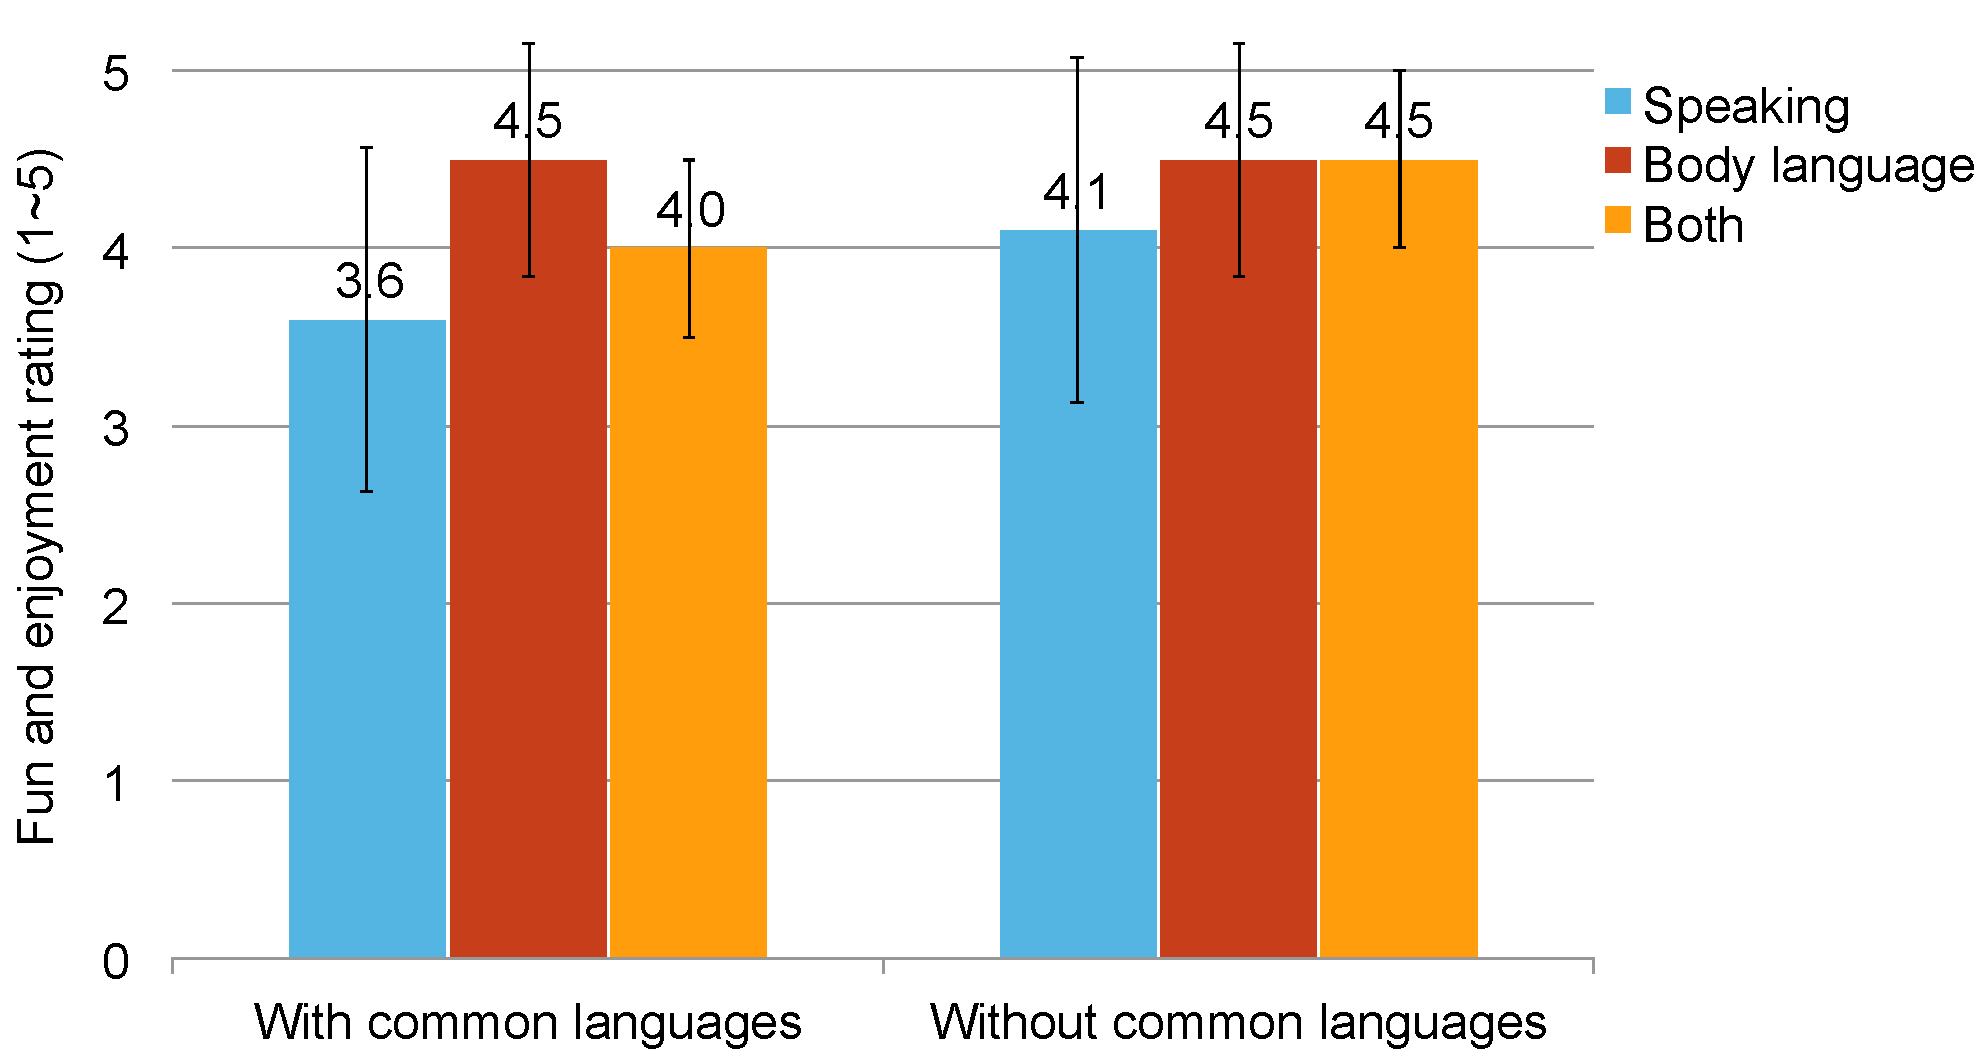
\includegraphics[width=0.9\columnwidth]{Figures/US_Fun.pdf}
\caption{eSFQ: fun/enjoyment rating for players \textit{with} and \textit{without} common languages.}
\label{fig:US_Fun}
\end{figure}


Figure~\ref{fig:US_Fun} shows the fun/enjoyment rating for players with and without common languages using the three communication modes. 
For players with common languages, their mean rating for Speaking mode was 3.58 (SD = 1.14), and the most popular keywords selected were ``simple'' (83\% of the users) and ``intuitive'' (54\%). 
Their mean rating for Body language mode was 4.54 (SD = 0.66), and the most popular keywords selected were ``intuitive'' (54\%), ``exciting'' (46\%) and ``great'' (42\%). 
Their mean rating for Both mode was 3.96 (SD = 1.00), and the most popular keywords selected were ``intuitive'' (63\%), ``simple'' (63\%) and ``exciting'' (33\%). 

For players without common languages (see Figure~\ref{fig:US_Fun}), 
their mean rating for Speaking mode was 4.08 (SD = 0.97), and the most popular keywords selected were ``great'' (42\% of the users), ``intuitive'' (38\%), ``simple'' (38\%), and ``confusing'' (33\%). 
Their mean rating for Body language mode was 4.46 (SD = 0.66), and the most popular keywords selected were ``intuitive'' (54\%), ``exciting'' (46\%), ``simple'' (38\%) and ``difficult'' (33\%). 
Their mean rating for Both mode was 4.50 (SD = 0.59). , and the most popular keywords selected were ``intuitive'' (67\%), ``exciting'' (42\%), ``simple'' (42\%), ``great'' (34\%) and ``confusing'' (33\%).


As we can see in Figure~\ref{fig:US_Fun}, the two communication modes with body language had higher fun/enjoyment ratings compared to the speaking-only mode for all players (both with and without common languages). 



\subsection{Positive and Negative Co-experience}

\begin{figure}[!t]
\centering
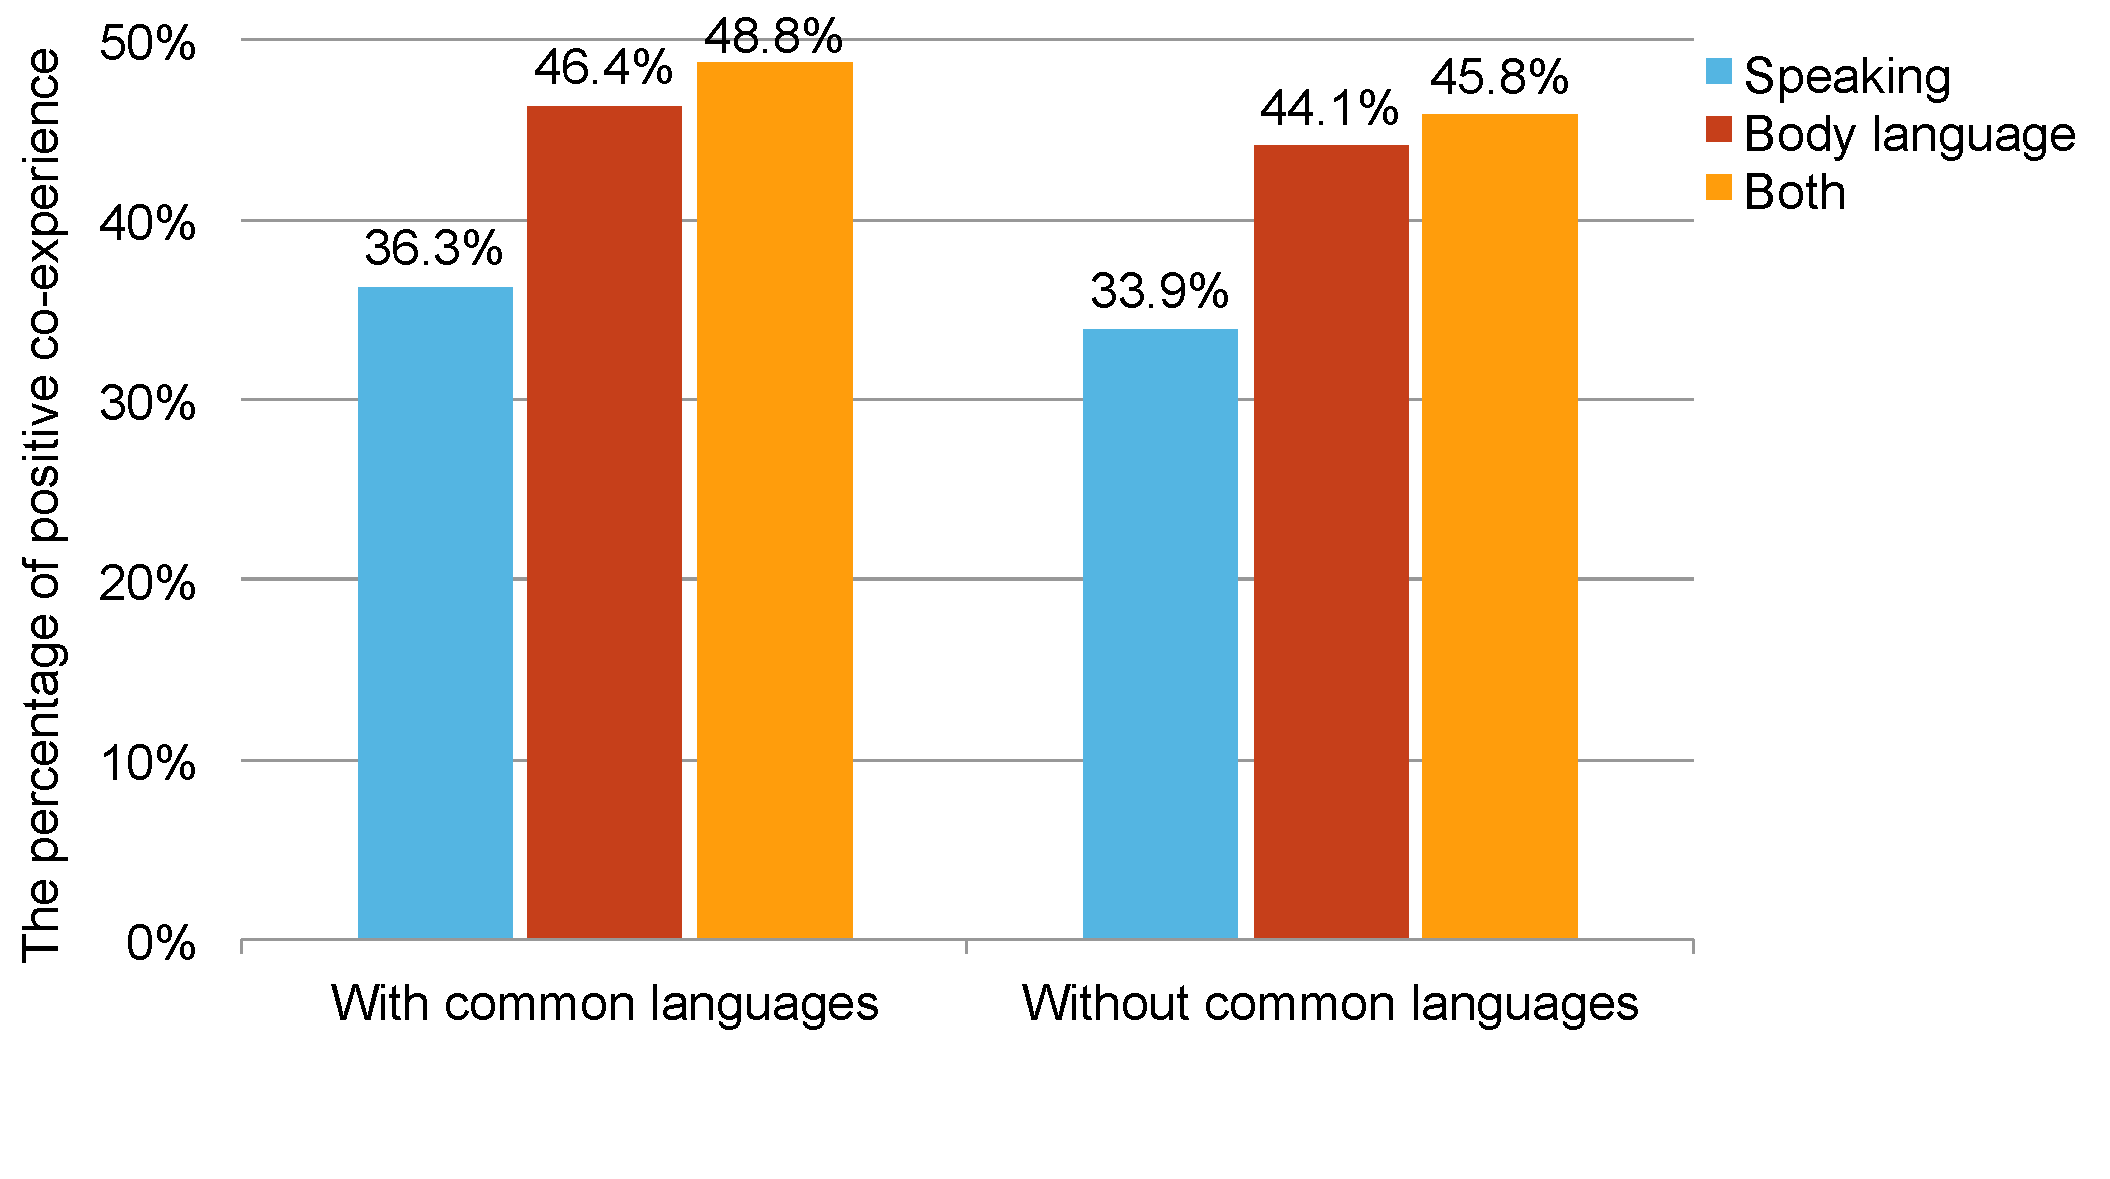
\includegraphics[width=0.8\columnwidth]{Figures/US_eSFQ_Pos_Average.pdf}
\caption{eSFQ: average co-experience of positive indexes (Cooperative, Happy, Fun, Fair, Encouraging, Triumphing, Satisfying).}
\label{fig:US_eSFQ_Pos_Average}
\end{figure}

\begin{figure}[!t]
\centering
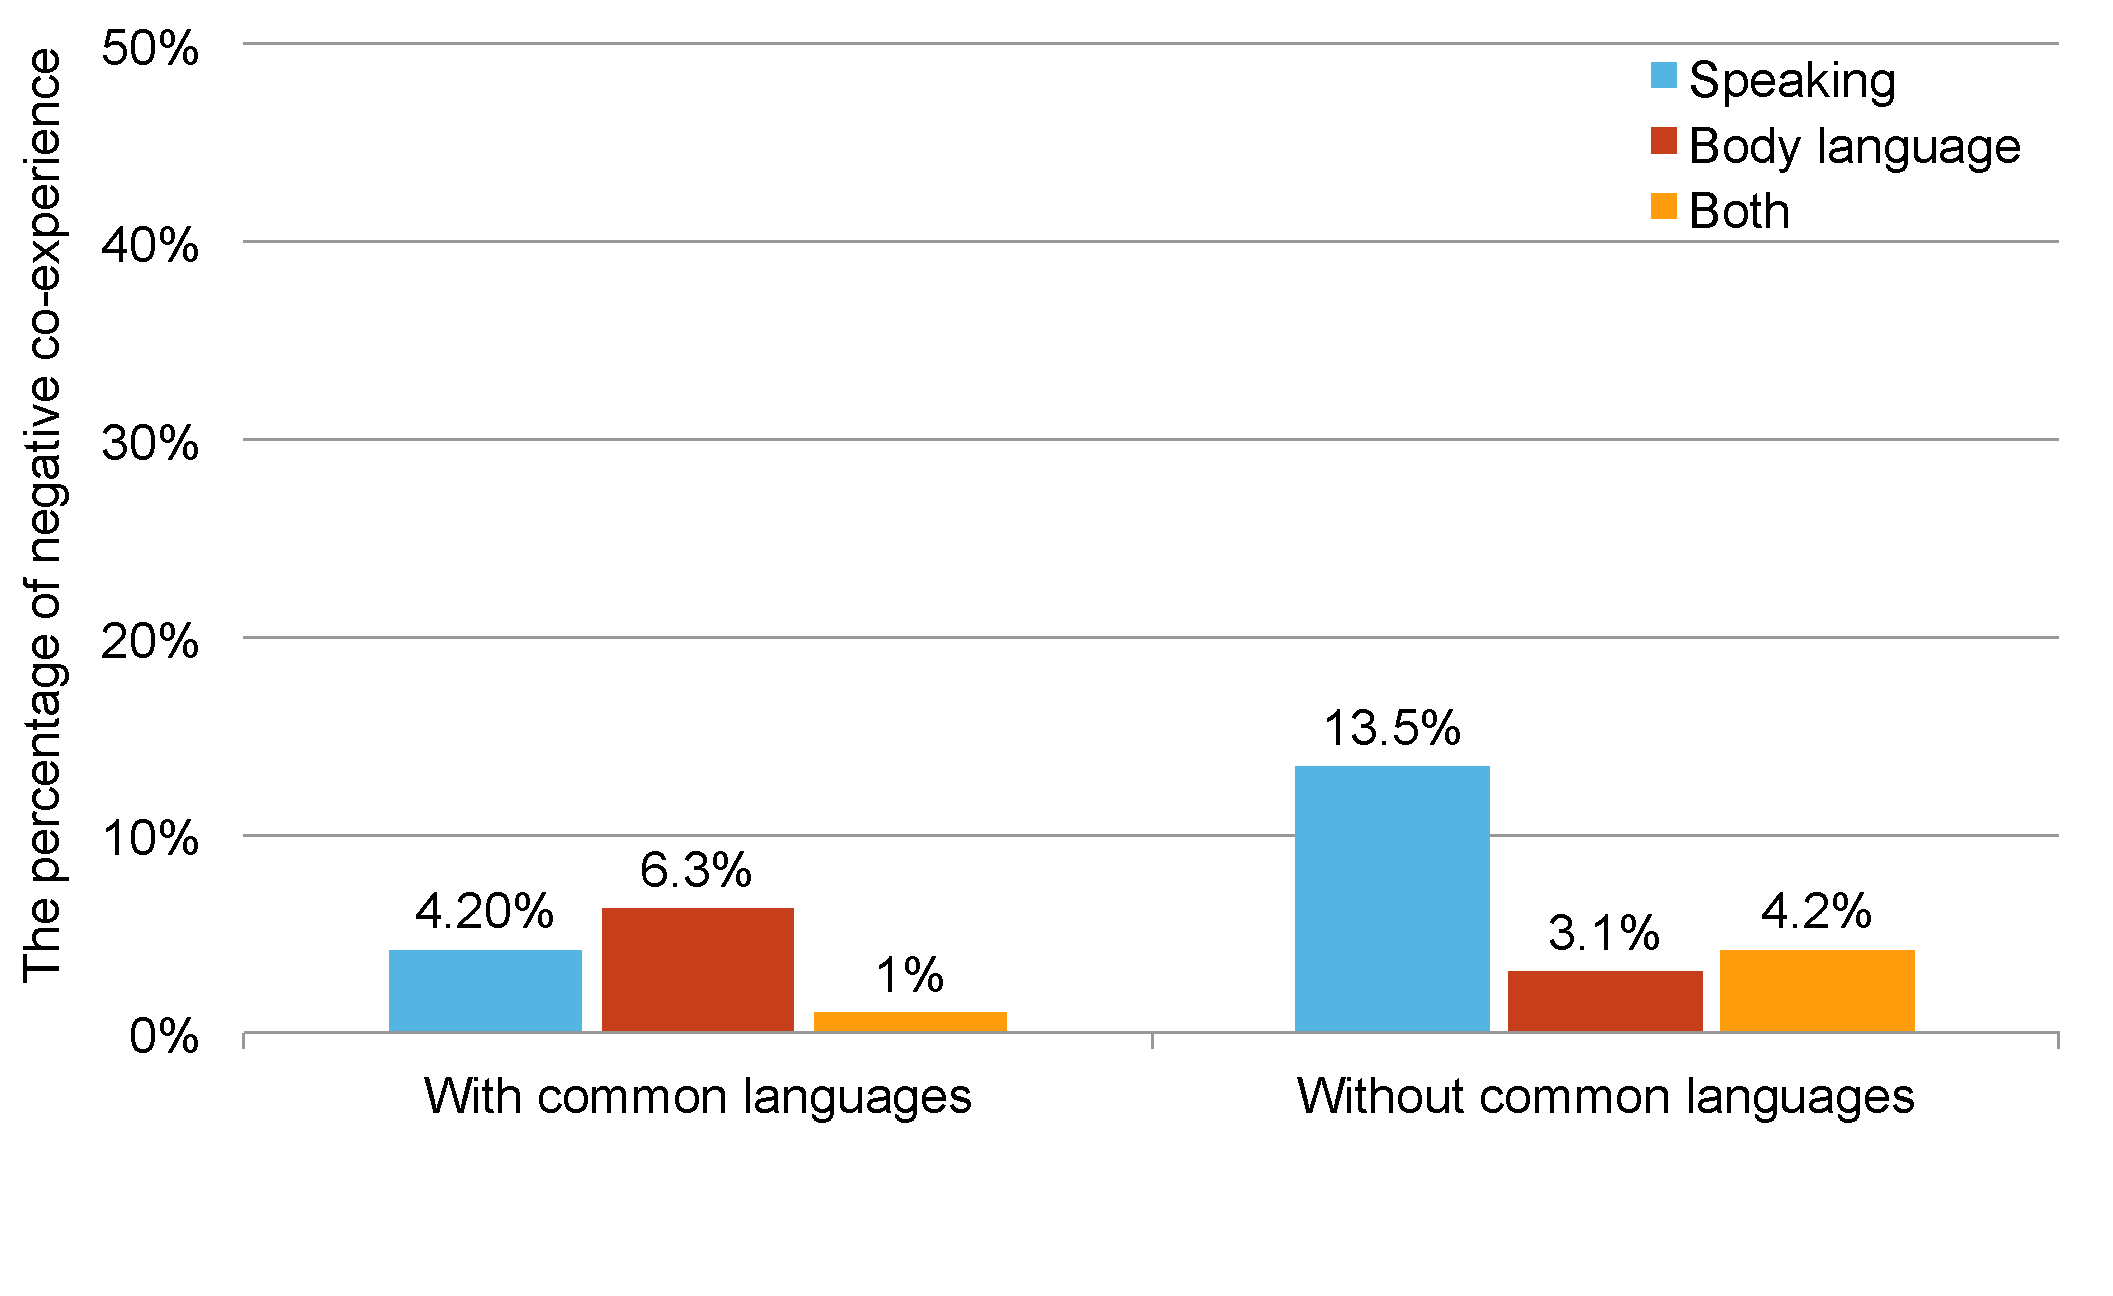
\includegraphics[width=0.8\columnwidth]{Figures/US_eSFQ_Neg_Average.pdf}
\caption{eSFQ: average co-experience of negative indexes (Defeat, Angry, Frustrating, Boring).}
\label{fig:US_eSFQ_Neg_Average}
\end{figure}


Figure~\ref{fig:US_eSFQ_Pos_Average} shows the average positive co-experience indexes for players with and without common languages. The positive co-experience is higher for communication modes with body language. Compared to speaking-only mode, adding body language 
improved positive co-experience by an average of 31\% and 33\% for players with and without common languages, respectively.

Figure~\ref{fig:US_eSFQ_Neg_Average} shows the average negative co-experience indexes for players with and without common languages. Compared to speaking-only mode, adding body language 
improved negative co-experience by an average of 13\% and 73\% for players with and without common languages, respectively.

\begin{figure}[!b]
\centering
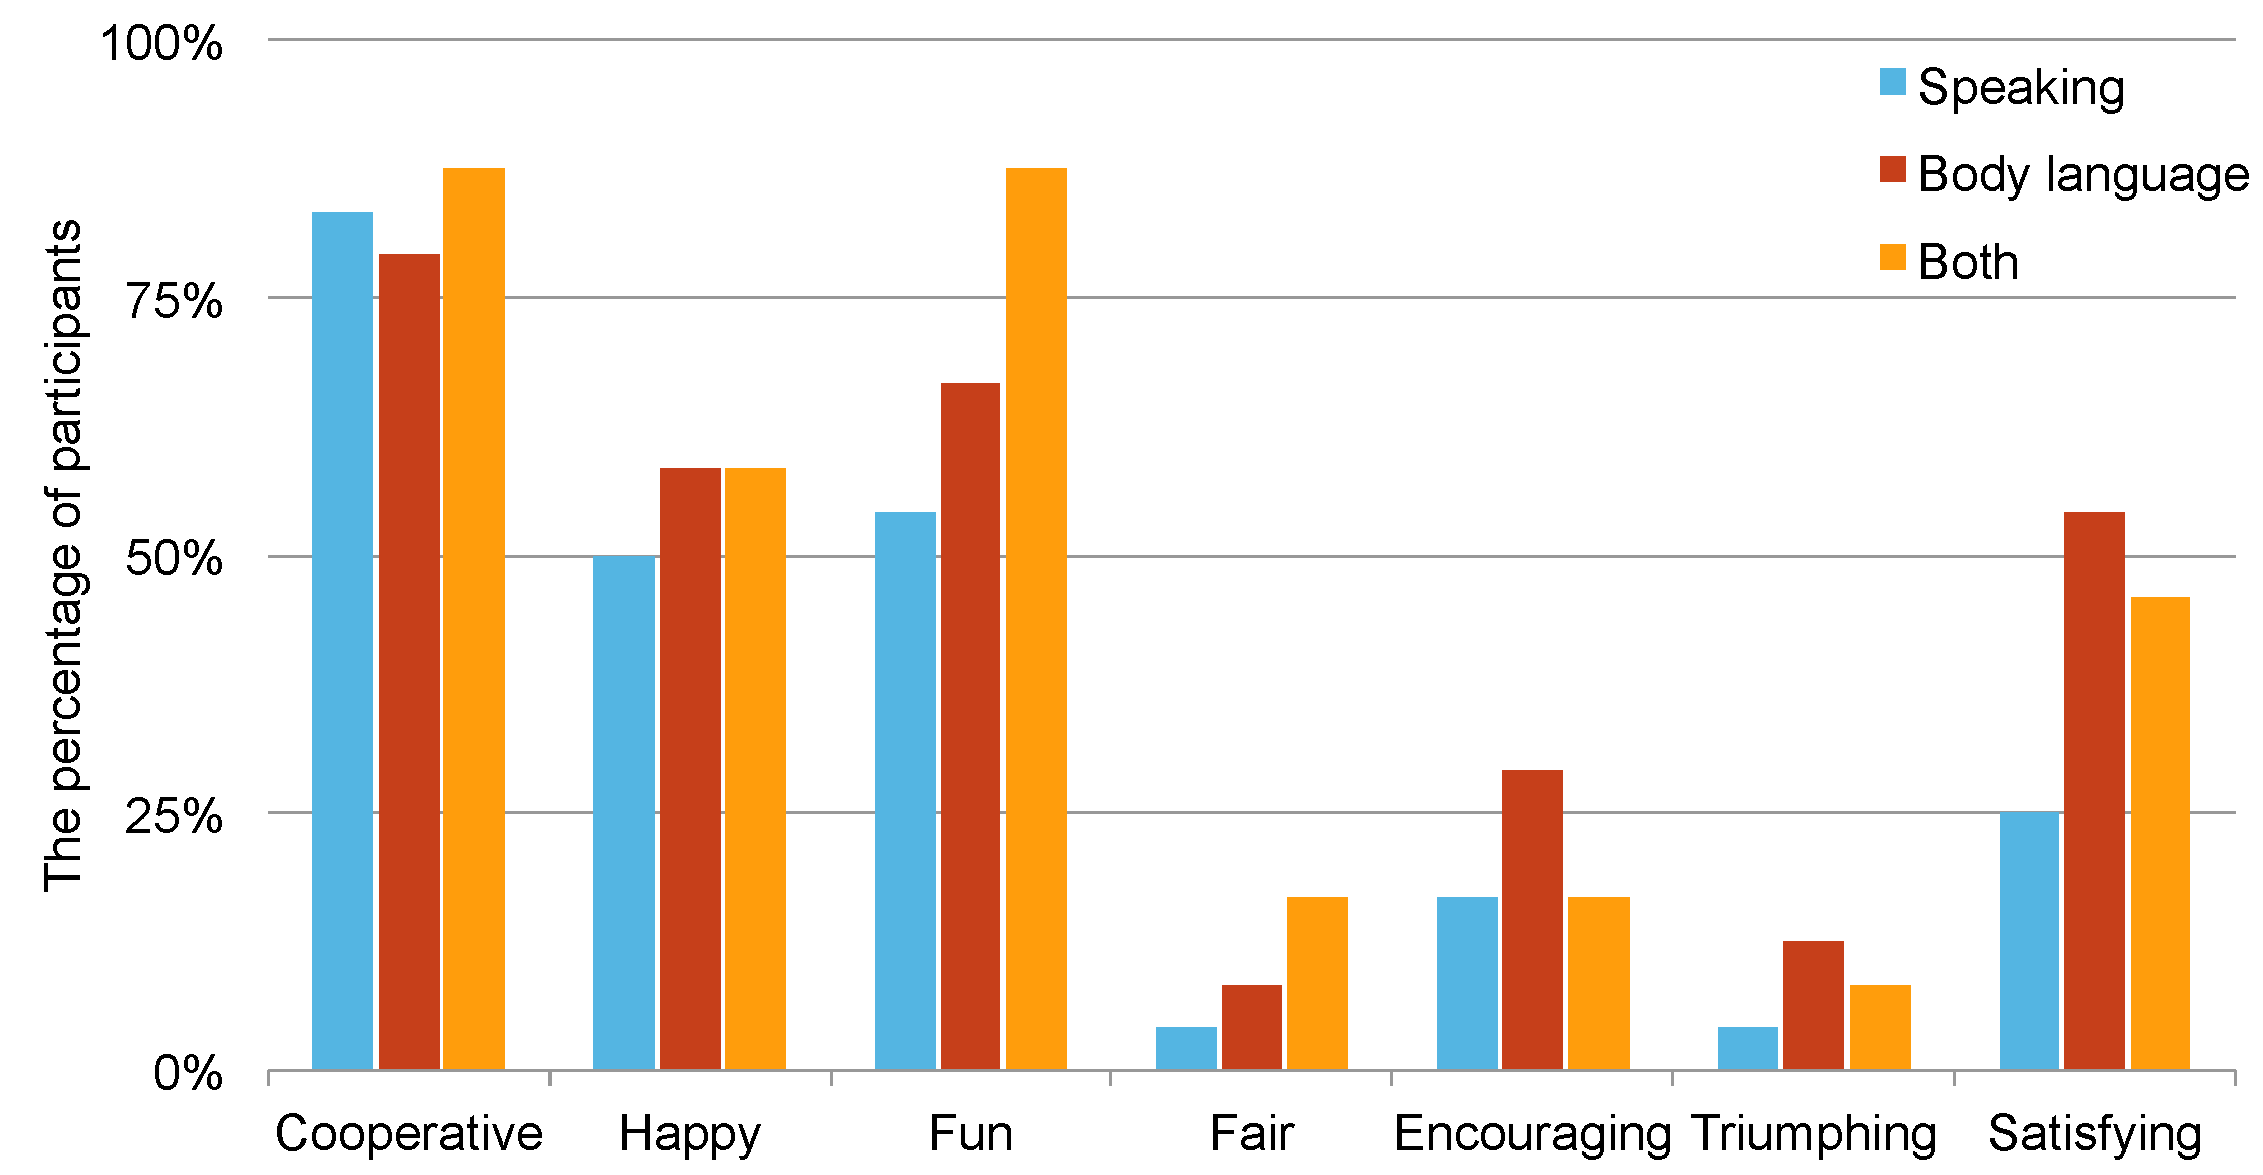
\includegraphics[width=0.9\columnwidth]{Figures/US_Co-ex_Dif_Pos.pdf}
\caption{Positive co-experience indexes for players without common languages.}
\label{fig:US_Co-ex_Dif_Pos}
\end{figure}

\begin{figure}[!t]
\centering
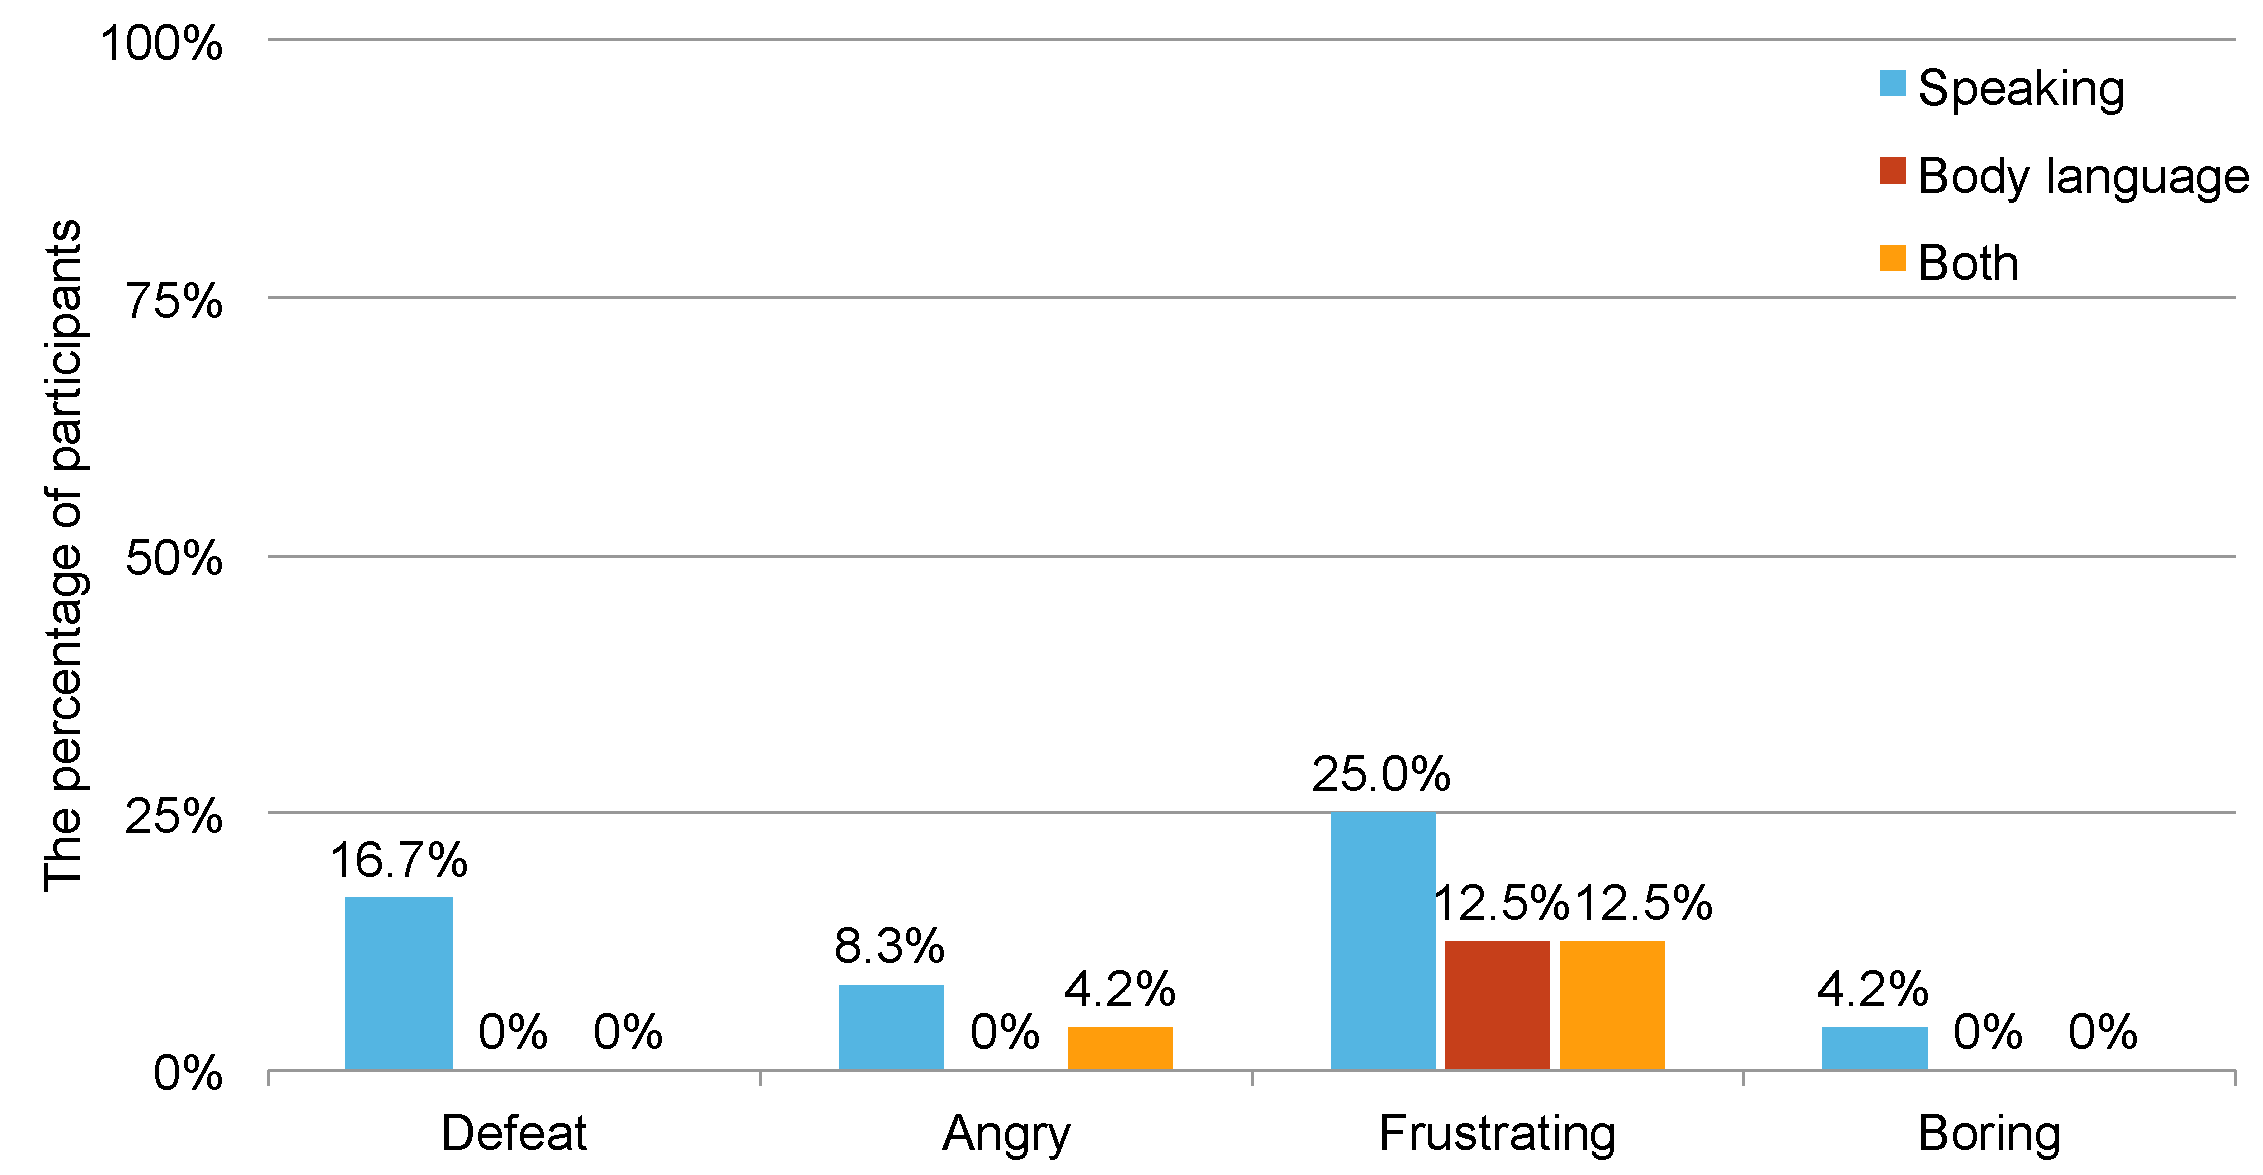
\includegraphics[width=0.9\columnwidth]{Figures/US_Co-ex_Dif_Neg.pdf}
\caption{Negative co-experience indexes for players without common languages (lower is better).}
\label{fig:US_Co-ex_Dif_Neg}
\end{figure}

Figure~\ref{fig:US_Co-ex_Dif_Pos} shows the individual positive co-experience indexes for players without common languages. Compared to speaking-only mode, we can see that all of these positive indexes increase when body language is added (except for cooperative in body language only mode). Specifically, satisfaction improved by an average of 99.5\%. 


Figure~\ref{fig:US_Co-ex_Dif_Neg} shows the individual negative co-experience indexes for players without common languages. Compared to speaking-only mode, we can see that all of these negative indexes decrease when body language is added. Specifically, defeat and boring dropped from 16.7\% to zero, and frustration improved by an average of 48\%. 

\section{Cooperative Performance Metrics (CPM) Results}

Cooperative Performance Metrics (CPM)\cite{CPMs} is designed to analyze cooperative gaming experience, typically through manual coding of the video recordings of players' facial expression (e.g. laughter) and body movement. CPM counts the occurrences of the following six types of co-behavior: ``Laughter or excitement together'', ``Work out strategies'', ``Helping each other'', ``Global Strategies'', ``Waited for each other'' and ``Got in each other's way ''.
Because `Global Strategies'' and ``Got in each other's way'' do not apply to our game, they are not shown in the subsequent analysis.

Before we started coding CPMs, we performed a formal validation process to ensure inter-rater consistency. We asked two independent researchers to understand CPMs in depth and were shown examples of how to apply them using video of a gameplay session. Afterwards, researchers were given four videos to analyze and we calculated inter-rater agreement using kappa values\cite{Kappa1,Kappa2}. 

%Table~\ref{tab:KappaValue} shows the results of our validation
We calculated the kappa values for each metric and for each of the sample videos. The lowest Kappa value, 0.75, is greater than 0.6 and is sufficient to establish validity. To further ensure accurate coding of CPMs, each of the 24-pairs of user study sessions was coded by oth researchers, and the results were averaged. 


% \begin{table}[!h]
% \renewcommand\arraystretch{1.2}
%   \centering
%   \begin{tabular}{
%   !{\vrule width2pt}m{0.15\columnwidth}
%   !{\vrule width2pt}m{0.15\columnwidth}
%   !{\vrule width2pt}m{0.17\columnwidth}
%   !{\vrule width2pt}m{0.15\columnwidth}
%   !{\vrule width2pt}m{0.15\columnwidth}
%   !{\vrule width2pt}}
%     \hline
%     \multicolumn{1}
%     {!{\vrule width2pt}c!{\vrule width2pt}}
%     {\tabhead{\multirow{2}{*}{Inter-rater}}} &
%     \multicolumn{4}
%     {c!{\vrule width2pt}}
%     {\centering\tabhead{Kappa for Metrics}} \\
%     \Xcline{2-5}{2pt}
%      & Laughter together & Work out strategies & Helping each other & Waited for each other\\
%     \hline
%     Session1 & 0.75 & 1 & 0.79 & 1\\
%     \hline
%     Session2 & 1 & 0.8 & 1 & 1\\
%     \hline
%     Session3 & 0.75 & 1 & 0.87 & 1\\
%     \hline
%     Session4 & 1 & 1 & 0.96 & 1\\
%     \hline
%     Average & 0.88 & 0.96 & 0.91 & 1\\
%     \hline
%   \end{tabular}
%   \caption{Inter-rater Agreement (M stands for CPM)}
%   \label{tab:KappaValue}
% \end{table}


\begin{figure}[!h]
\centering
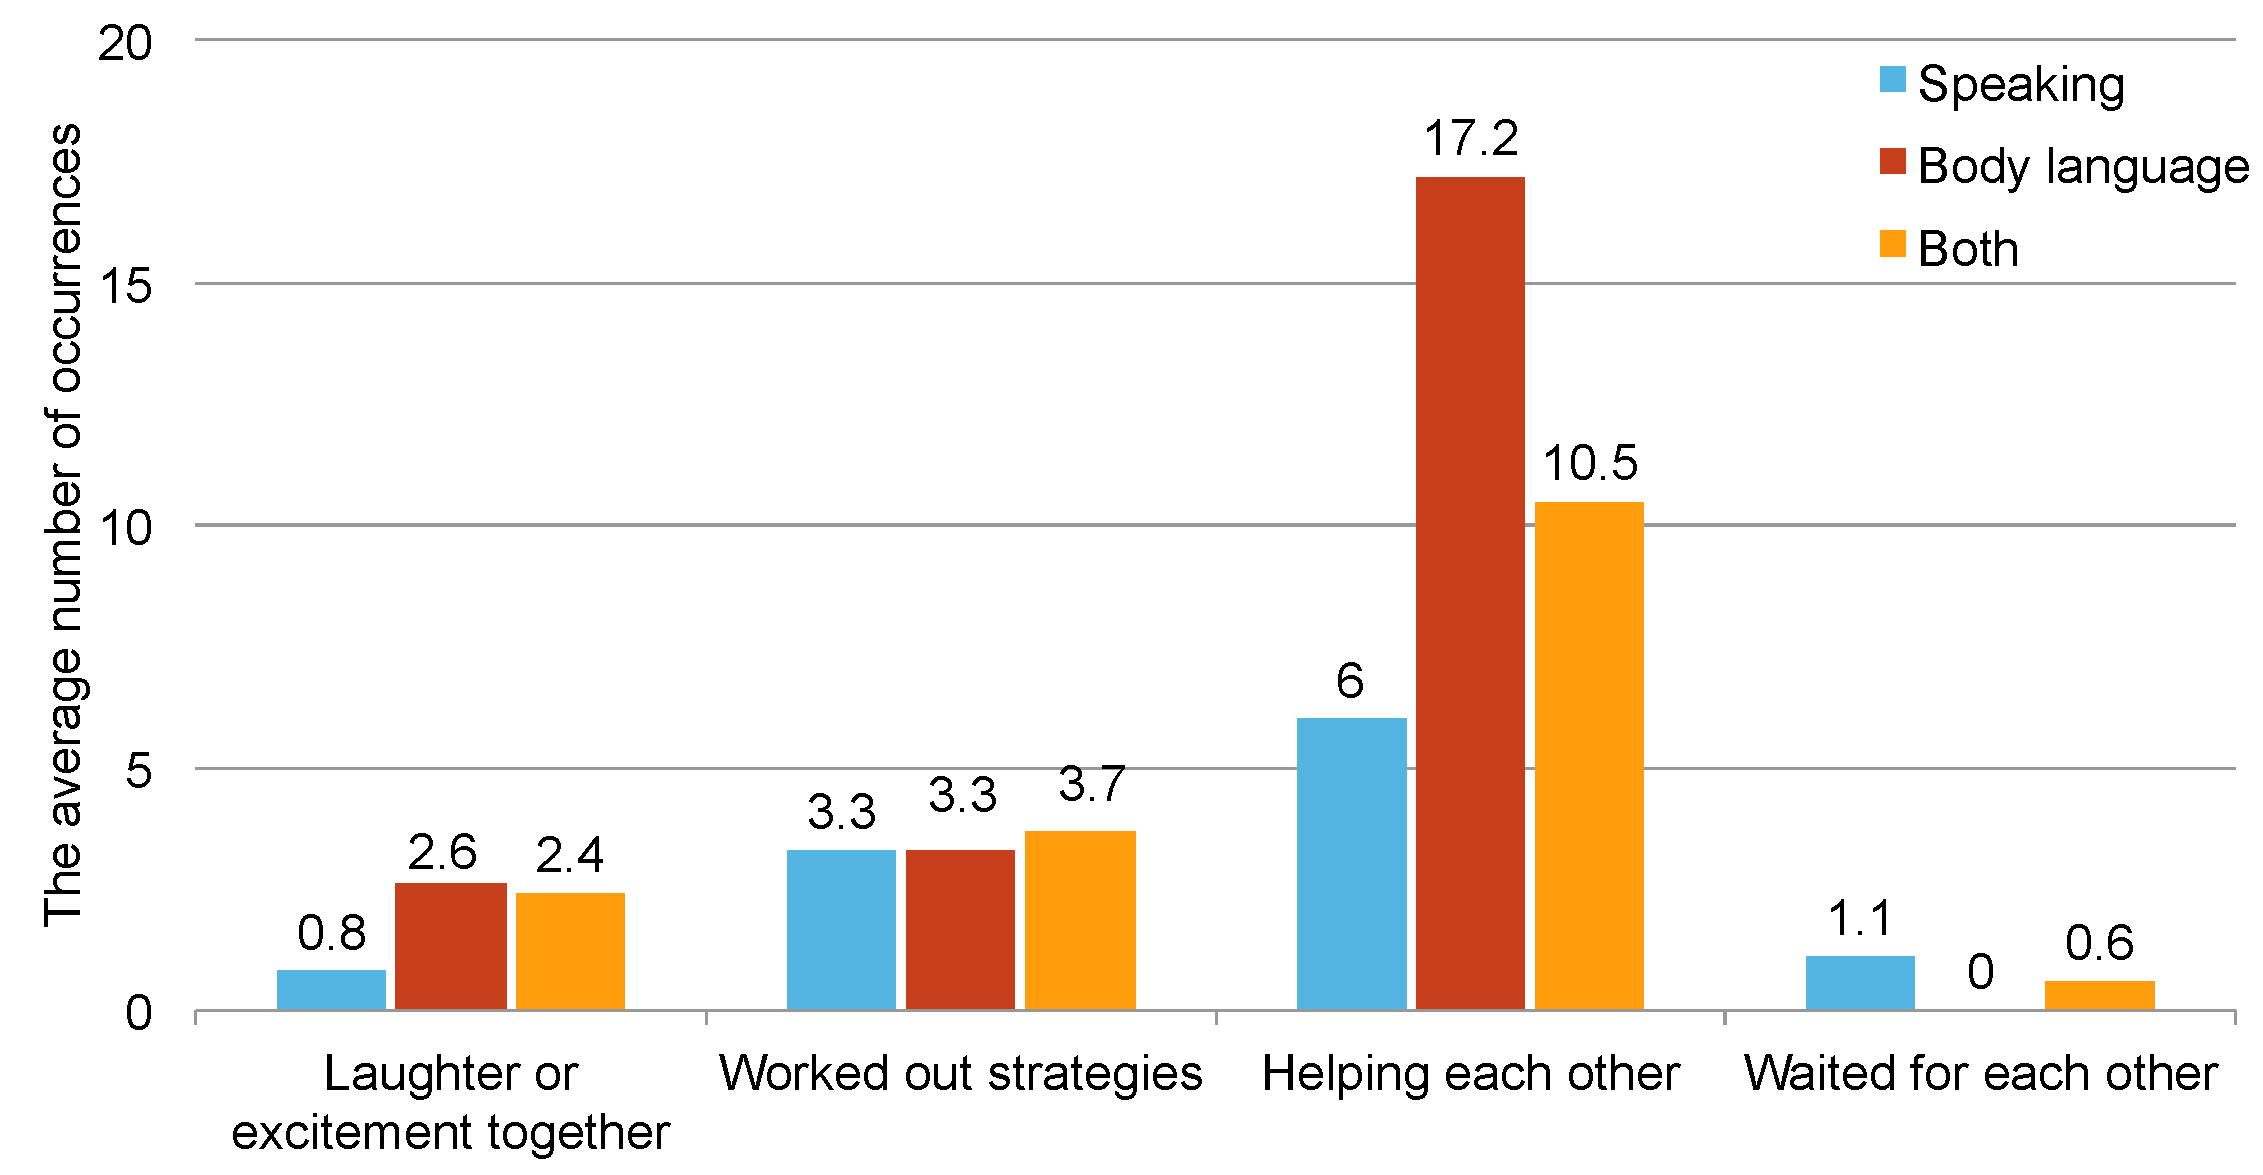
\includegraphics[width=0.9\columnwidth]{Figures/US_CPMs_Com.pdf}
\caption{CPMs result for players with common languages.}
\label{fig:US_CPMs_Com}
\end{figure}

\begin{figure}[!h]
\centering
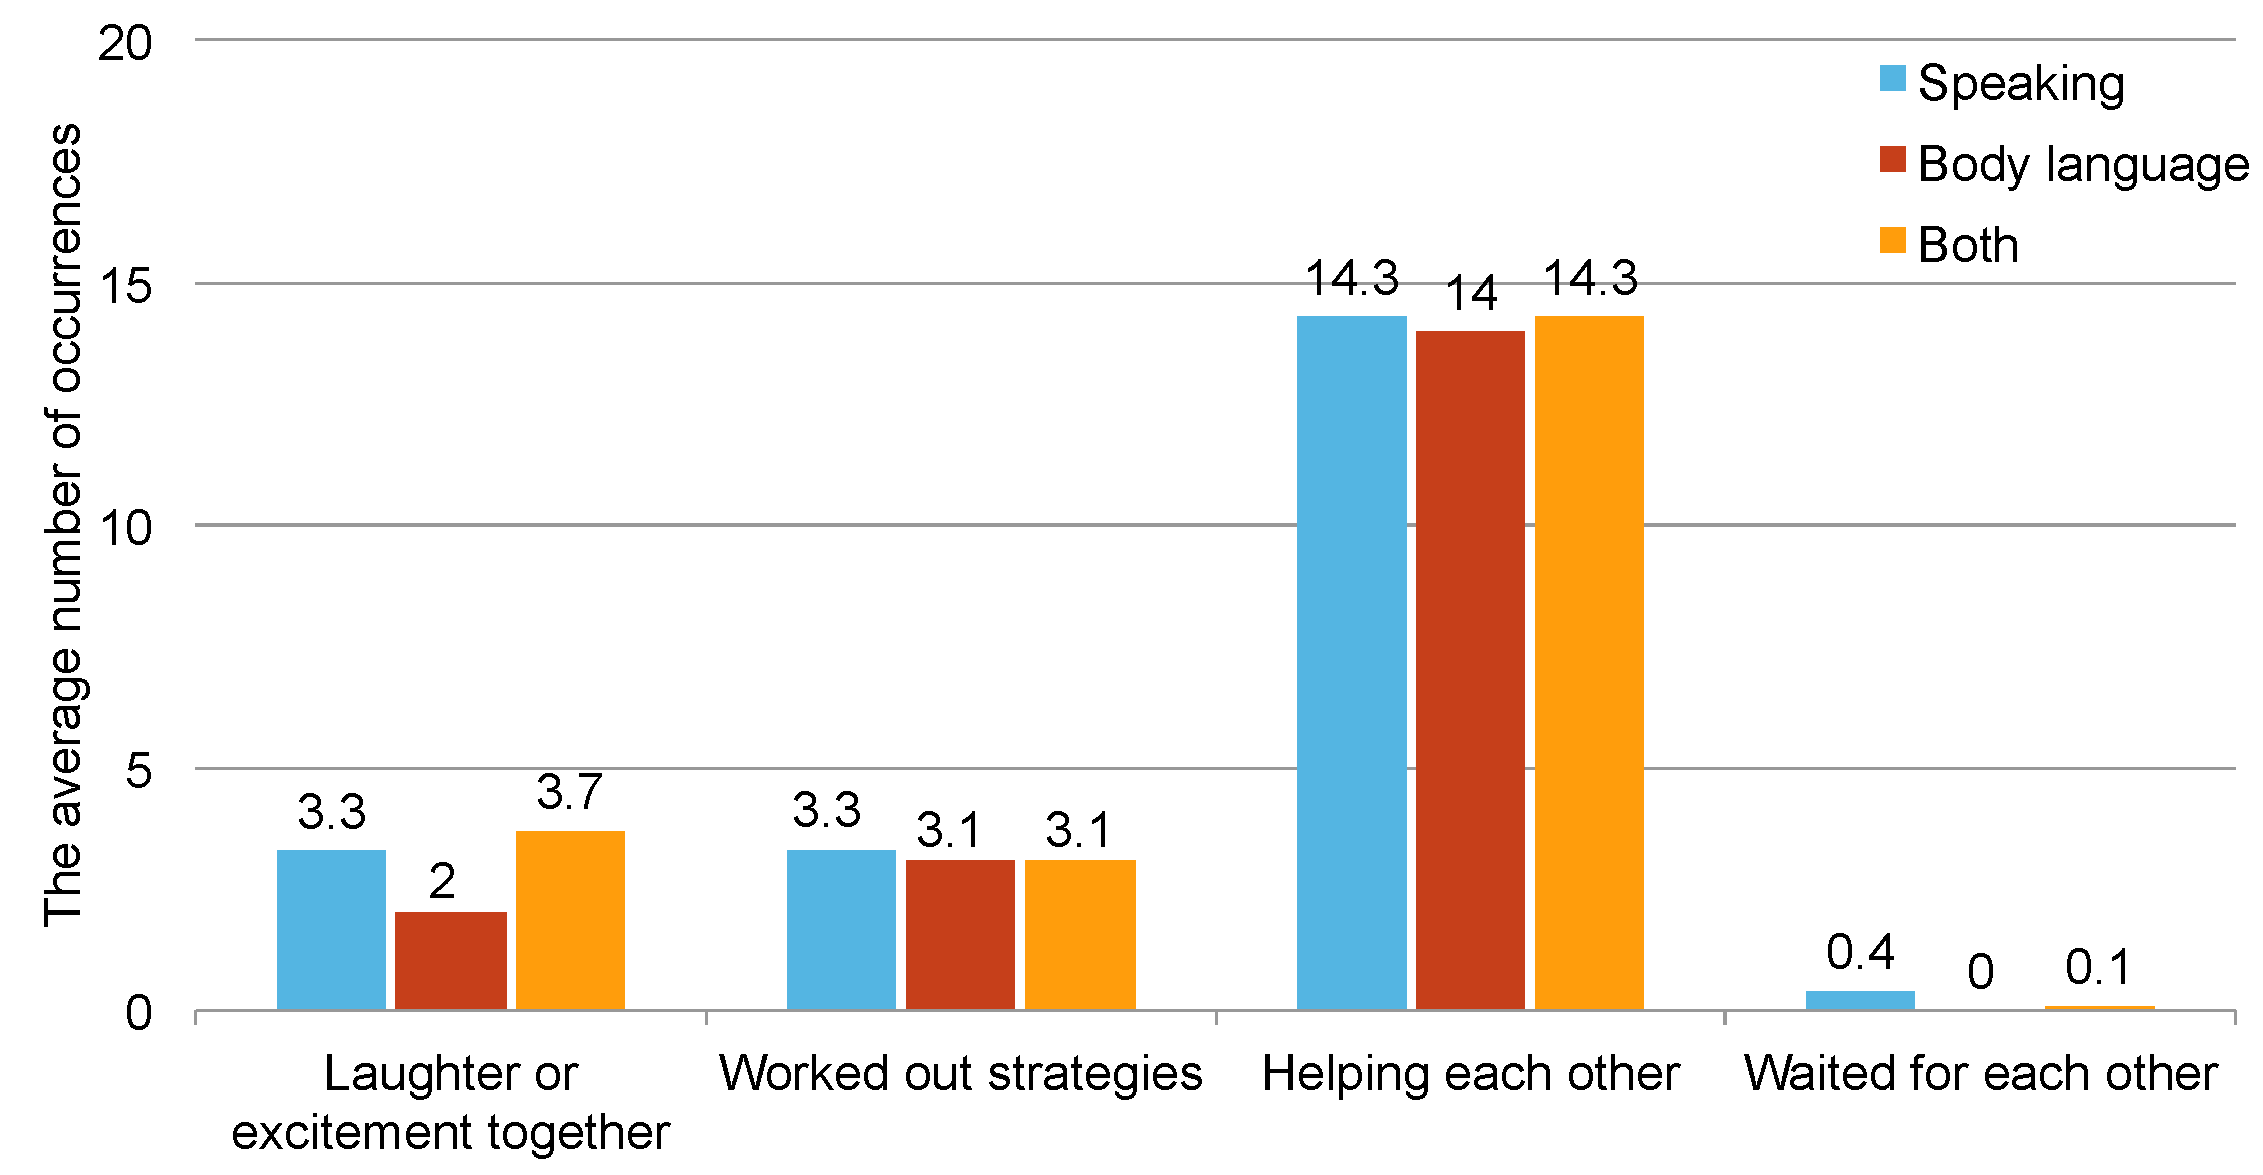
\includegraphics[width=0.9\columnwidth]{Figures/US_CPMs_Dif.pdf}
\caption{CPMs result for players without common languages.}
\label{fig:US_CPMs_Dif}
\end{figure}

Figure~\ref{fig:US_CPMs_Com} shows the CPM results for players with common languages. Compared to speaking only, adding body language communication increased ``laughter or excitement'' and ``helping each other''. ``Laughter or excitement'' increased because body language sometime led to unexpected and funny body movement. ``Helping each other'' increased because players were communicating with shorter but more frequent instructions, leading to more occurrences of helping each other being recorded. 

Figure~\ref{fig:US_CPMs_Dif} shows the CPM results for players without common languages. 
``Laughter or excitement'' was lowest for the body language mode.  We observed funny sounds and tones the players would make, such as when someone fumbled and made a clumsy mistake, and would lead to laughter. Also, laughter by one player was often mirrored by the other player. 


\section{Final Questionnaire Results}
Our final questionnaire asked the preferences among the communication modes: ``Favorite'', ``Most fun'', ``Easiest'', ``Most difficult'', ``Most intuitive'', and ``Most cooperative''.


\begin{figure}[!t]
\centering
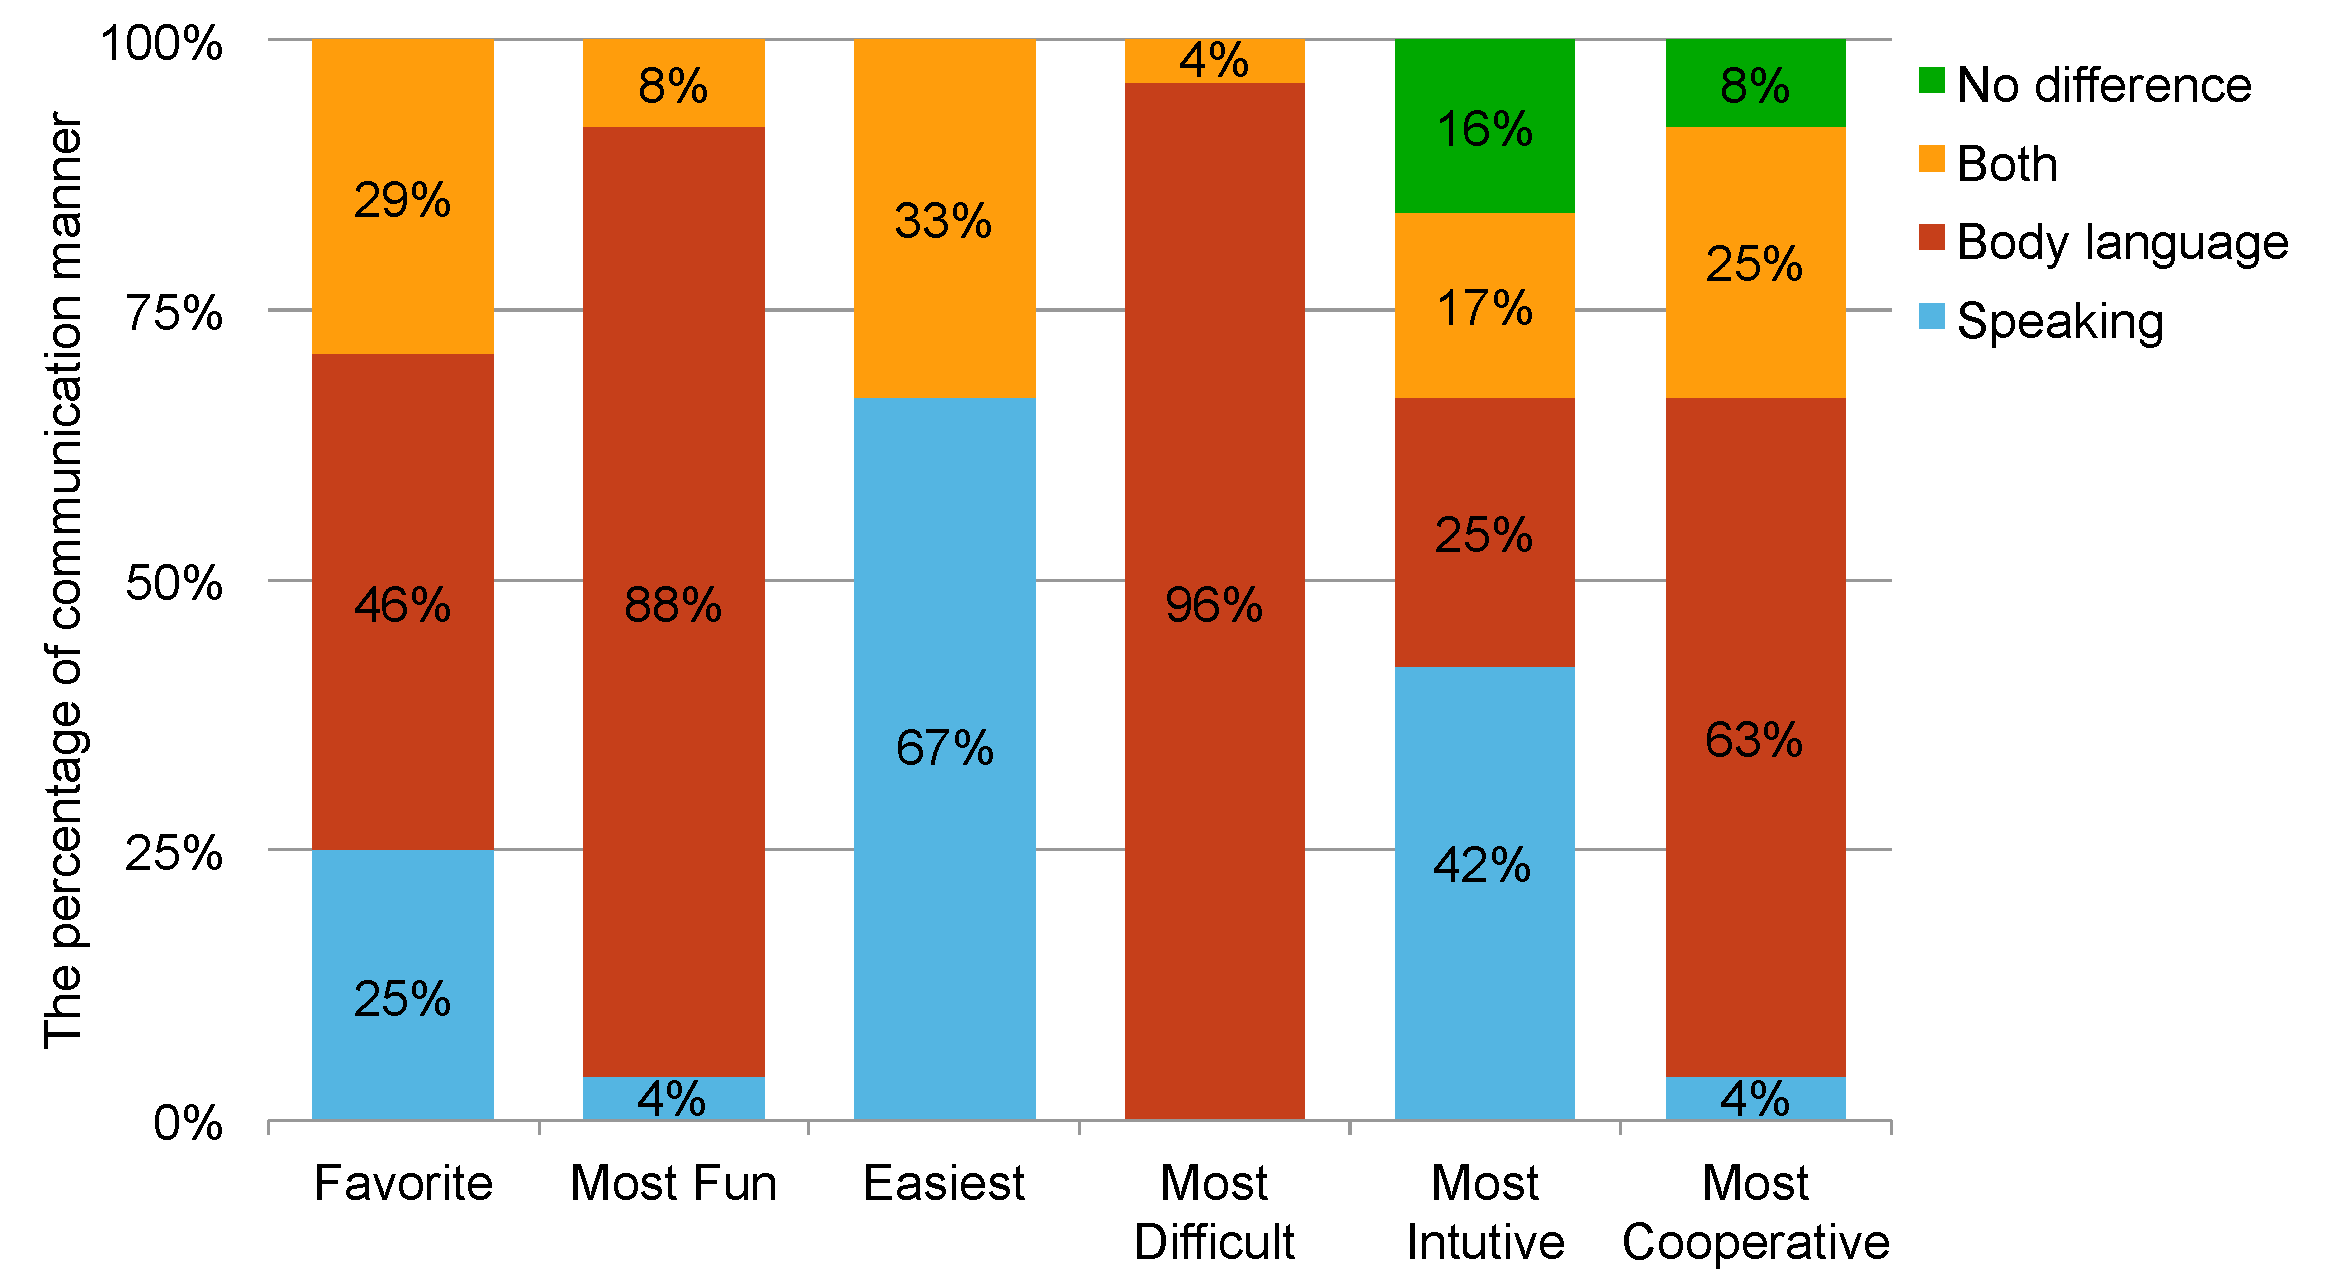
\includegraphics[width=0.9\columnwidth]{Figures/US_FQ_Com.pdf}
\caption{Overall preference for players with common languages.}
\label{fig:US_FQ_Com}
\end{figure}

Figure~\ref{fig:US_FQ_Com} shows the preferences for players with common languages. 
Body language without speaking was found to be most difficult by 96\% of the players, yet had the highest proportion in the index of ``Favorite'' (46\%), ``Most fun'' (88\%), and ``Most cooperative'' (63\%). Using the GameFlow model shown in Figure~\ref{fig:GD_F1}, the experience in speaking mode may be boring, and the body language mode may lower the skill level and make the experience more fun.

\begin{figure}[!t]
\centering
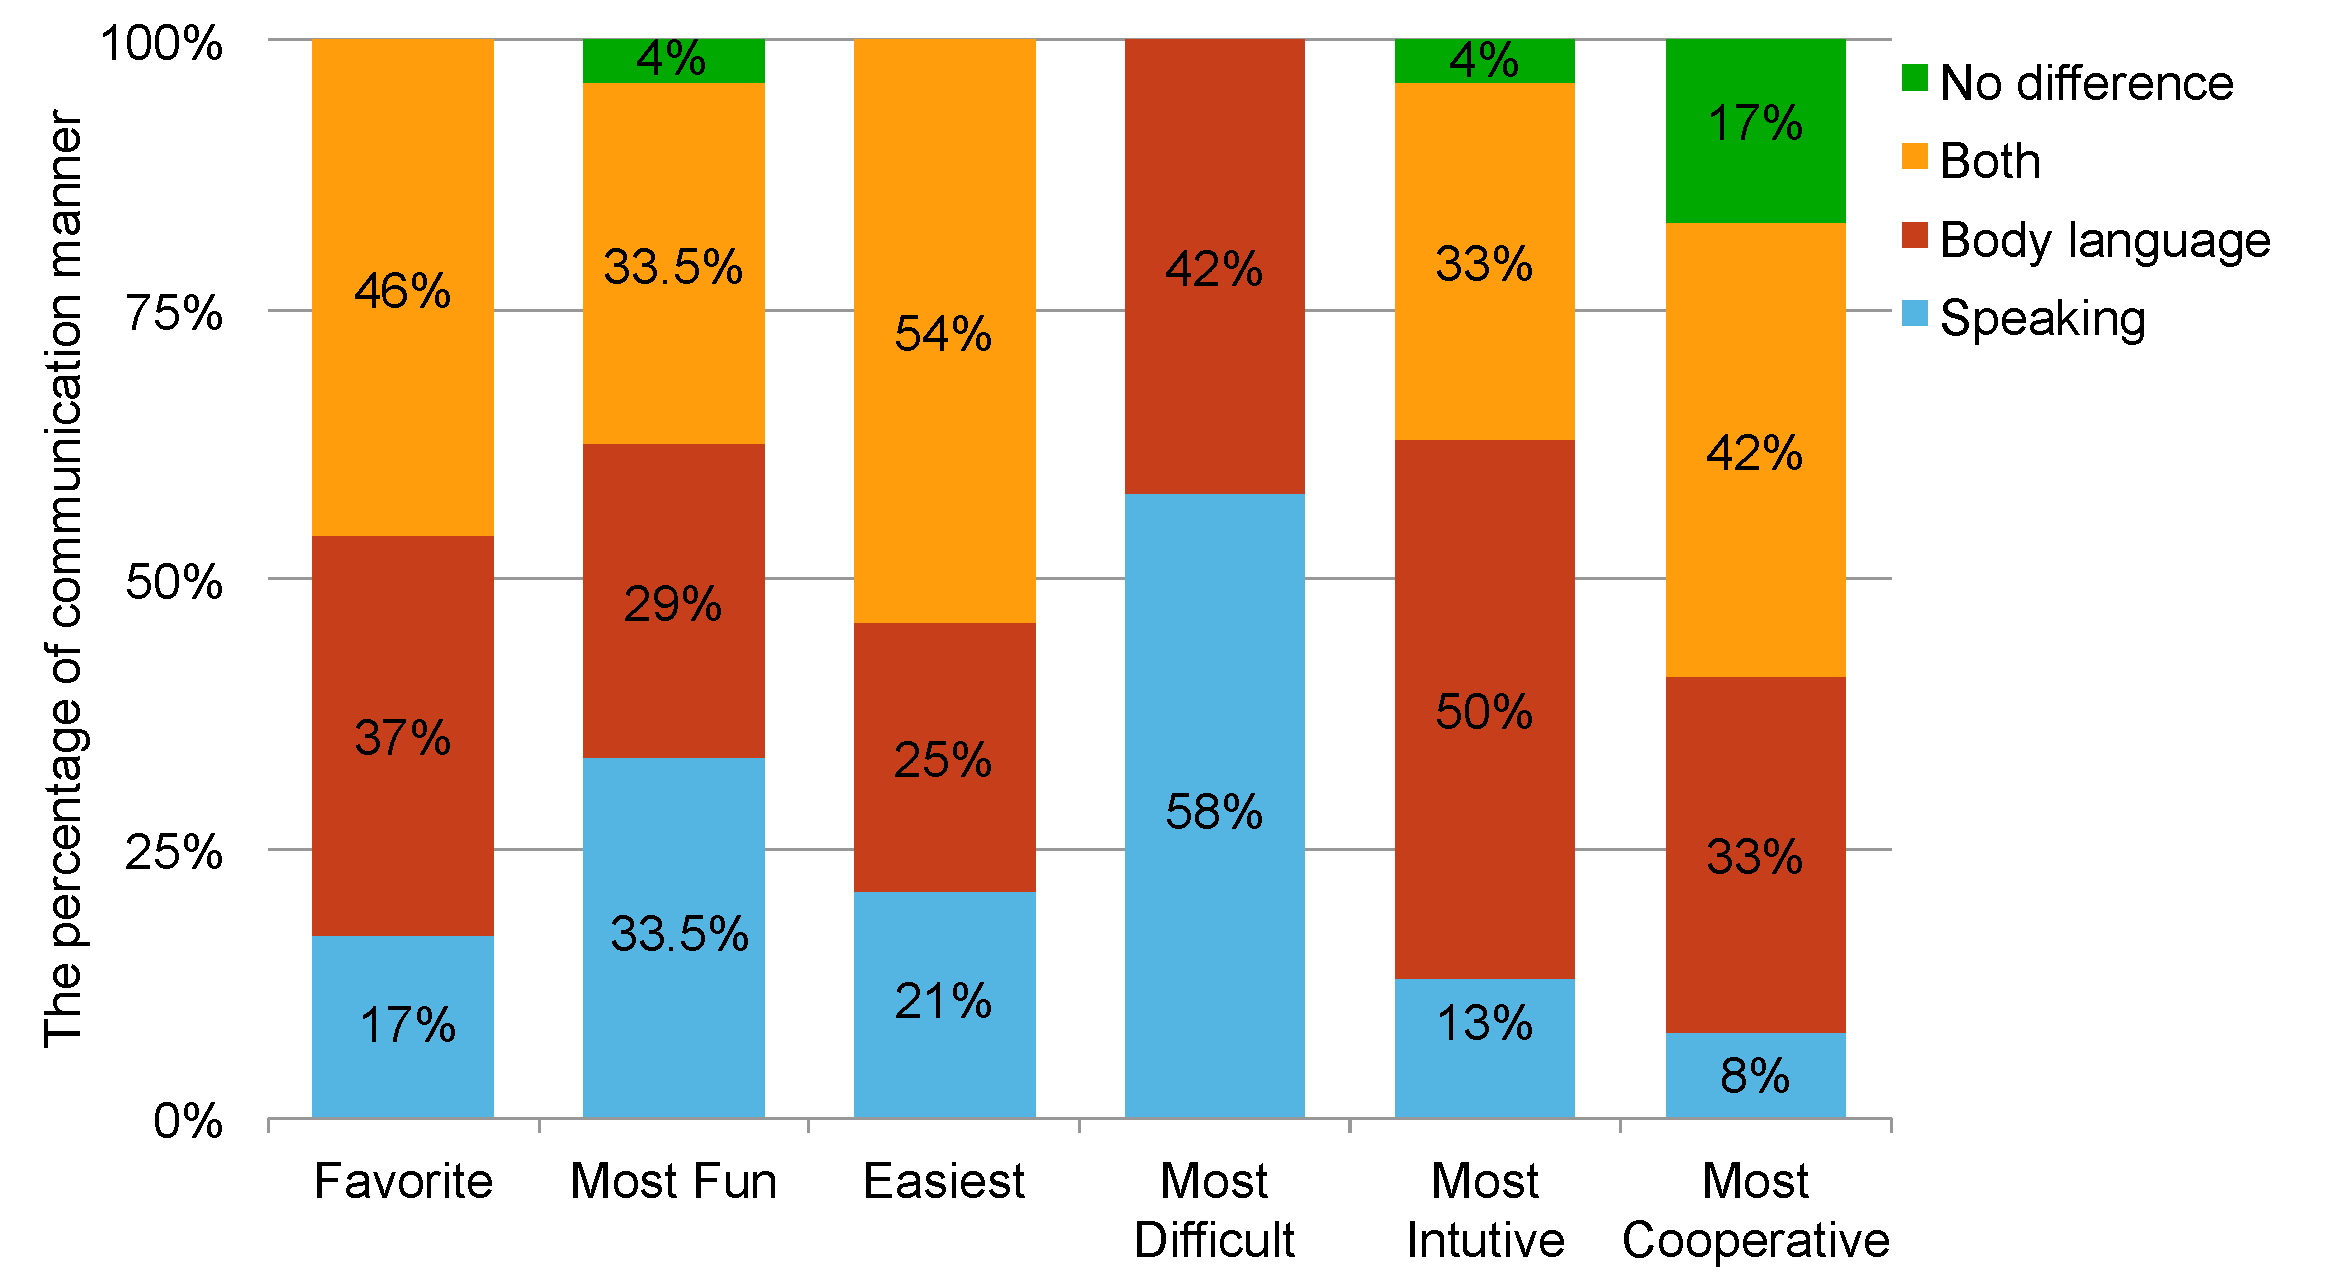
\includegraphics[width=0.9\columnwidth]{Figures/US_FQ_Dif.pdf}
\caption{Overall preference for players without common languages.}
\label{fig:US_FQ_Dif}
\end{figure}

Figure~\ref{fig:US_FQ_Dif} shows the preferences for players without common languages.
Most of the users (58\%) found the speaking mode as the most difficult, and found the body-language mode as the most intuitive (50\%). Most users preferred using both speaking and body language together (46\%) and found it ``Most fun'' (33.5\%), ``Easiest'' (54\%), and ``Most cooperative'' (42\%).

